\documentclass{beamer}
\usepackage[brazil]{babel}
\usepackage[utf8]{inputenc}
\usepackage[T1]{fontenc}
\usepackage{graphicx}
\usepackage{array}
\usepackage{listings}
\usepackage{url}
\usepackage{multicol}


%%%%%%%%%%%%%%%%%%%%%%%%%%%%%%%%%%%%%%%%%%%%%%%%%%%%%%%%%%%%%%%%%%%%%%%%%%%%%%%%
%
%  \zoombox[box line width]{contents}
%
%  optimized version for beamer: in full screen, zoom boxes are centred
%  in the viewer; useable with any documenclass
%
%%%%%%%%%%%%%%%%%%%%%%%%%%%%%%%%%%%%%%%%%%%%%%%%%%%%%%%%%%%%%%%%%%%%%%%%%%%%%%%%
\makeatletter
\newsavebox\zb@x
\newcounter{z@@m}
\usepackage{calc}
\newdimen\B@r\newdimen\P@r
\newdimen\@zw\newdimen\@zh\newdimen\@zd

\newcommand{\zoombox}[2][0]{%
  \leavevmode%
  \sbox\zb@x{#2}%
  \setlength\B@r{1pt*\ratio{\wd\zb@x}{\ht\zb@x+\dp\zb@x}}%
  \setlength\P@r{1pt*\ratio{\paperwidth}{\paperheight}}%
  \ifdim\B@r>\P@r\relax%
    \setlength\@zw{\wd\zb@x}\setlength\@zh{\@zw*\ratio{\paperheight}{\paperwidth}}%
    \setlength\@zd{(\@zh-\ht\zb@x-\dp\zb@x)*\real{0.5}+\dp\zb@x}%
    \setlength\@zh{\@zh-\@zd}%
  \else%
    \setlength\@zh{\ht\zb@x+\dp\zb@x}%
    \setlength\@zw{\@zh*\ratio{\paperwidth}{\paperheight}}%
    \setlength\@zh{\ht\zb@x}\setlength\@zd{\dp\zb@x}%
  \fi%
  \makebox[0pt][l]{\makebox[\wd\zb@x][c]{\makebox[\@zw][l]{%
    \pdfdest name {zbfs\thez@@m} fitr
      width  \@zw\space
      height \@zh\space
      depth  \@zd\space
  }}}%
  \pdfdest name {zb\thez@@m} fitr
    width  \wd\zb@x\space
    height \ht\zb@x\space
    depth  \dp\zb@x\space
  \immediate\pdfannot 
    width  \wd\zb@x\space
    height \ht\zb@x\space
    depth  \dp\zb@x\space
  {%
    /Subtype/Link/H/N
    /Border [0 0 #1 [1 2]]
    /A <<
      /S/JavaScript
      /JS (
        if(typeof(zoomed)=='undefined'||!zoomed){
          var lastView=this.viewState;
          if(app.fs.isFullScreen) this.gotoNamedDest('zbfs\thez@@m');
          else this.gotoNamedDest('zb\thez@@m');
          zoomed=true;
        }else{
          this.viewState=lastView;
          zoomed=false;
        }
      )
    >>
  }%
  \usebox{\zb@x}%
  \stepcounter{z@@m}%
} 
\makeatother
%%%%%%%%%%%%%%%%%%%%%%%%%%%%%%%%%%%%%%%%%%%%%%%%%%%%%%%%%%%%%%%%%%%%%%%%%%%%%%%


\usetheme{Laughlin}

\begin{document}
\title{Extracting Records from the Web Using a Signal Processing Approach}
%\author[Roberto Panerai Velloso]{Orientando: Roberto Panerai Velloso \\
%Orientadora: Carina F. Dorneles \\ \{rvelloso, dorneles\}@gmail.com }
\author[Roberto Panerai Velloso]{Roberto Panerai Velloso, Carina F. Dorneles \\ 
\{rvelloso, dorneles\}@gmail.com}
%\date{\today}
\date{}
%\institute{Universidade Federal de Santa Catarina}
\institute{
%UFSC - Universidade Federal de Santa Catarina \\ PPGCC - Programa de
% Pós-Graduação em Ciência da Computação
\begin{figure}[H]
  \label{fig:logo1}
    %
\includegraphics[scale=0.50]{img/brasao_ufsc_80.png}
    %
\includegraphics[scale=0.30]{img/brasao_418.png}
    
\includegraphics[scale=0.30]{img/cikm.png}
\end{figure}
%\begin{figure}[H]
%  \label{fig:logo2}
%    
\includegraphics[scale=0.30]{brasao_ufsc_80.png}
%\end{figure}
}

\frame{
\titlepage
} 

\frame{\frametitle{Table of Contents}
\begin{small}
\begin{multicols}{2}
  \tableofcontents
\end{multicols}
\end{small}
}

\section{Introduction}
%\frame{\tableofcontents[currentsection]}

\subsection{Context}
\frame{\frametitle{Context}
\begin{itemize}
\item History
\begin{itemize}
  \item about 15+ years of research on the subject;
  \item still an open problem (it is a hard one, indeed).
\end{itemize}
\item Extract structured data (\textit{i.e.}, relational) from semi-structured
sources.

\item Data is available for human consumption, not for machines.

\item Motivation
\begin{itemize}
  \item run (no)SQL queries over the data;
  \item assemble domain specific databases;
  \item enrich other applications with structured data.
\end{itemize}
\end{itemize}
}

\subsection{Problem}
\frame{\frametitle{Problem - Challenges}
\begin{itemize} 
	\item extraction from semi-structured sources;
	\item make use of syntactical information (our scope);
	\item scalability (large amount of data to be processed):
	\begin{itemize}
	  \item level of supervision;
	  \item generality (diversity of data);
	  \item precision vs recall.
\end{itemize}
\end{itemize}
}

\subsection{Contributions}
\frame{\frametitle{Contributions}
\begin{itemize}
  \item a novel insight on how the structure of a web document can be seen;
  \item a novel web page segmentation technique;
  \item a new and efficient way of checking if a given region of a web page is
    structured or not;
  \item a more efficient approach, when compared to the state-of-the-art,
    that is due to the use of efficient signal processing algorithms.
\end{itemize}
}

\section{Approach}

\subsection{Main Features}
\frame{\frametitle{Main Features}
\begin{itemize}
  \item domain independent;
  \item HTML independent; 
  \item unsupervised;
  \item needs only one input page for extraction;
  \item computationally efficient.
\end{itemize}
}

\subsection{Assumptions}
\frame{\frametitle{Assumptions}
\begin{enumerate}
\item \textbf{Segmantation}: 
different regions of a document have different formatting so one can distinguish
one region from another (regardless the presence of noise). Therefore they are
formed using different tag paths, otherwise the visual difference 
would not be enough to distinguish them.

\textbf{Records}: 
semi-structured regions are composed by a set of contiguous records with similar
structure (and, consequently, by similar tag paths), so the subsequence
that represents these regions should be cyclic.
\end{enumerate} 
}


\subsection{Overall diagram}
\frame{\frametitle{Overall diagram}
\begin{figure}[H]
  \centering
    \zoombox{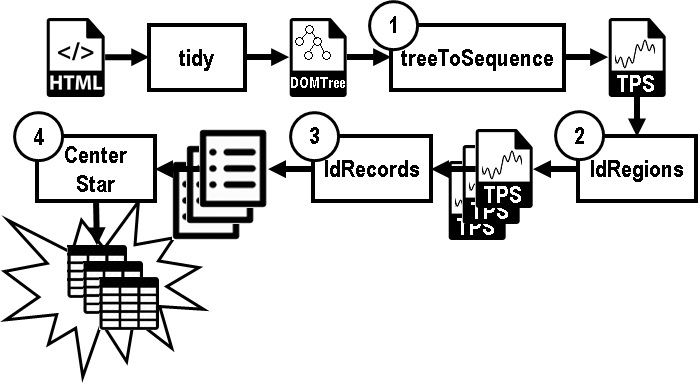
\includegraphics[width=1.00\textwidth]{img/proposal.jpg}}
\end{figure}
}

\subsection{Tag Paths}
\frame{\frametitle{$Tag$ $paths$}
\begin{figure}[H]
  \caption{Tag Path Sequence construction.}
  \centering
    \zoombox{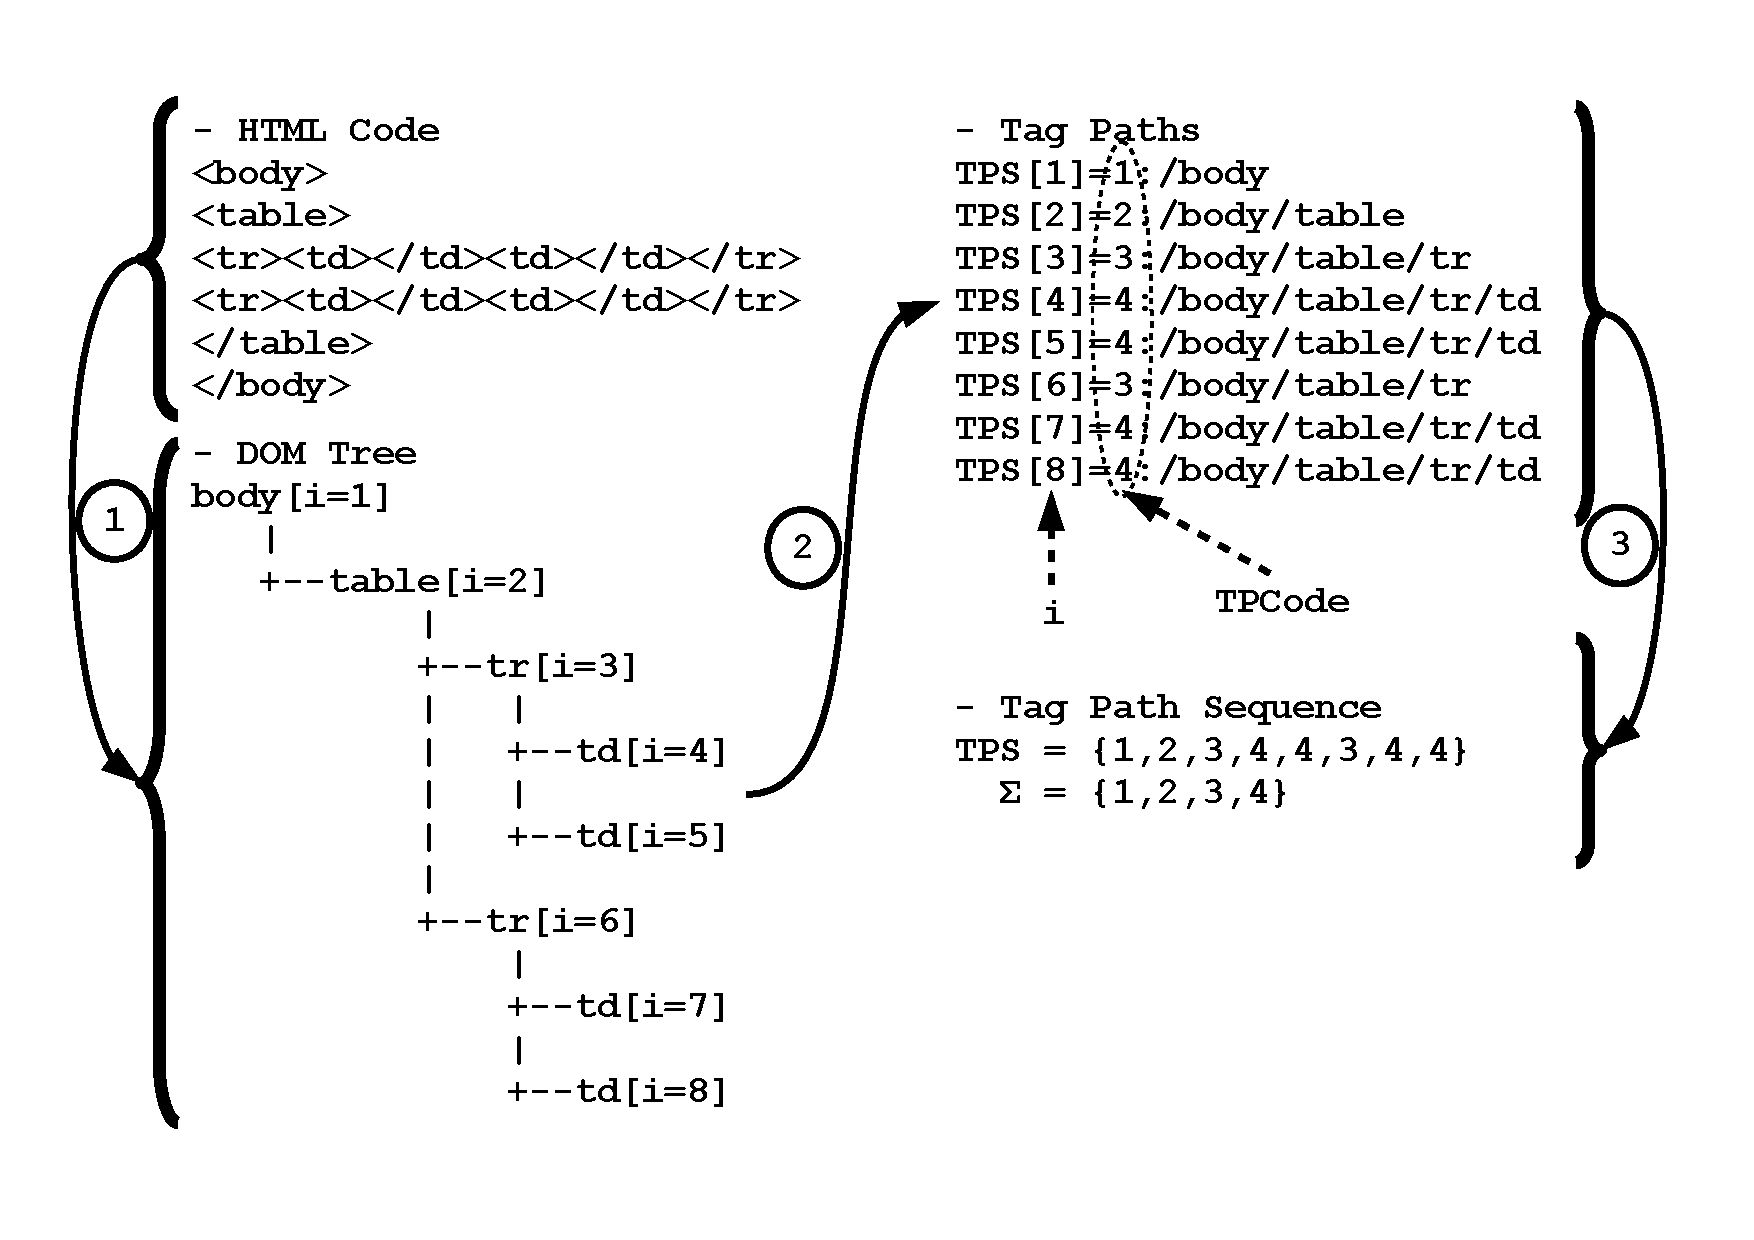
\includegraphics[clip, trim={1.1cm 1.9cm 1.5cm 1.65cm},
    width=1.00\textwidth]{img/tree2seq.pdf}}
\end{figure}
}
\frame{\frametitle{$Tag$ $paths$}
\begin{figure}[H]
  \caption{Tag Path Sequence document representation.}
  \centering
    \zoombox{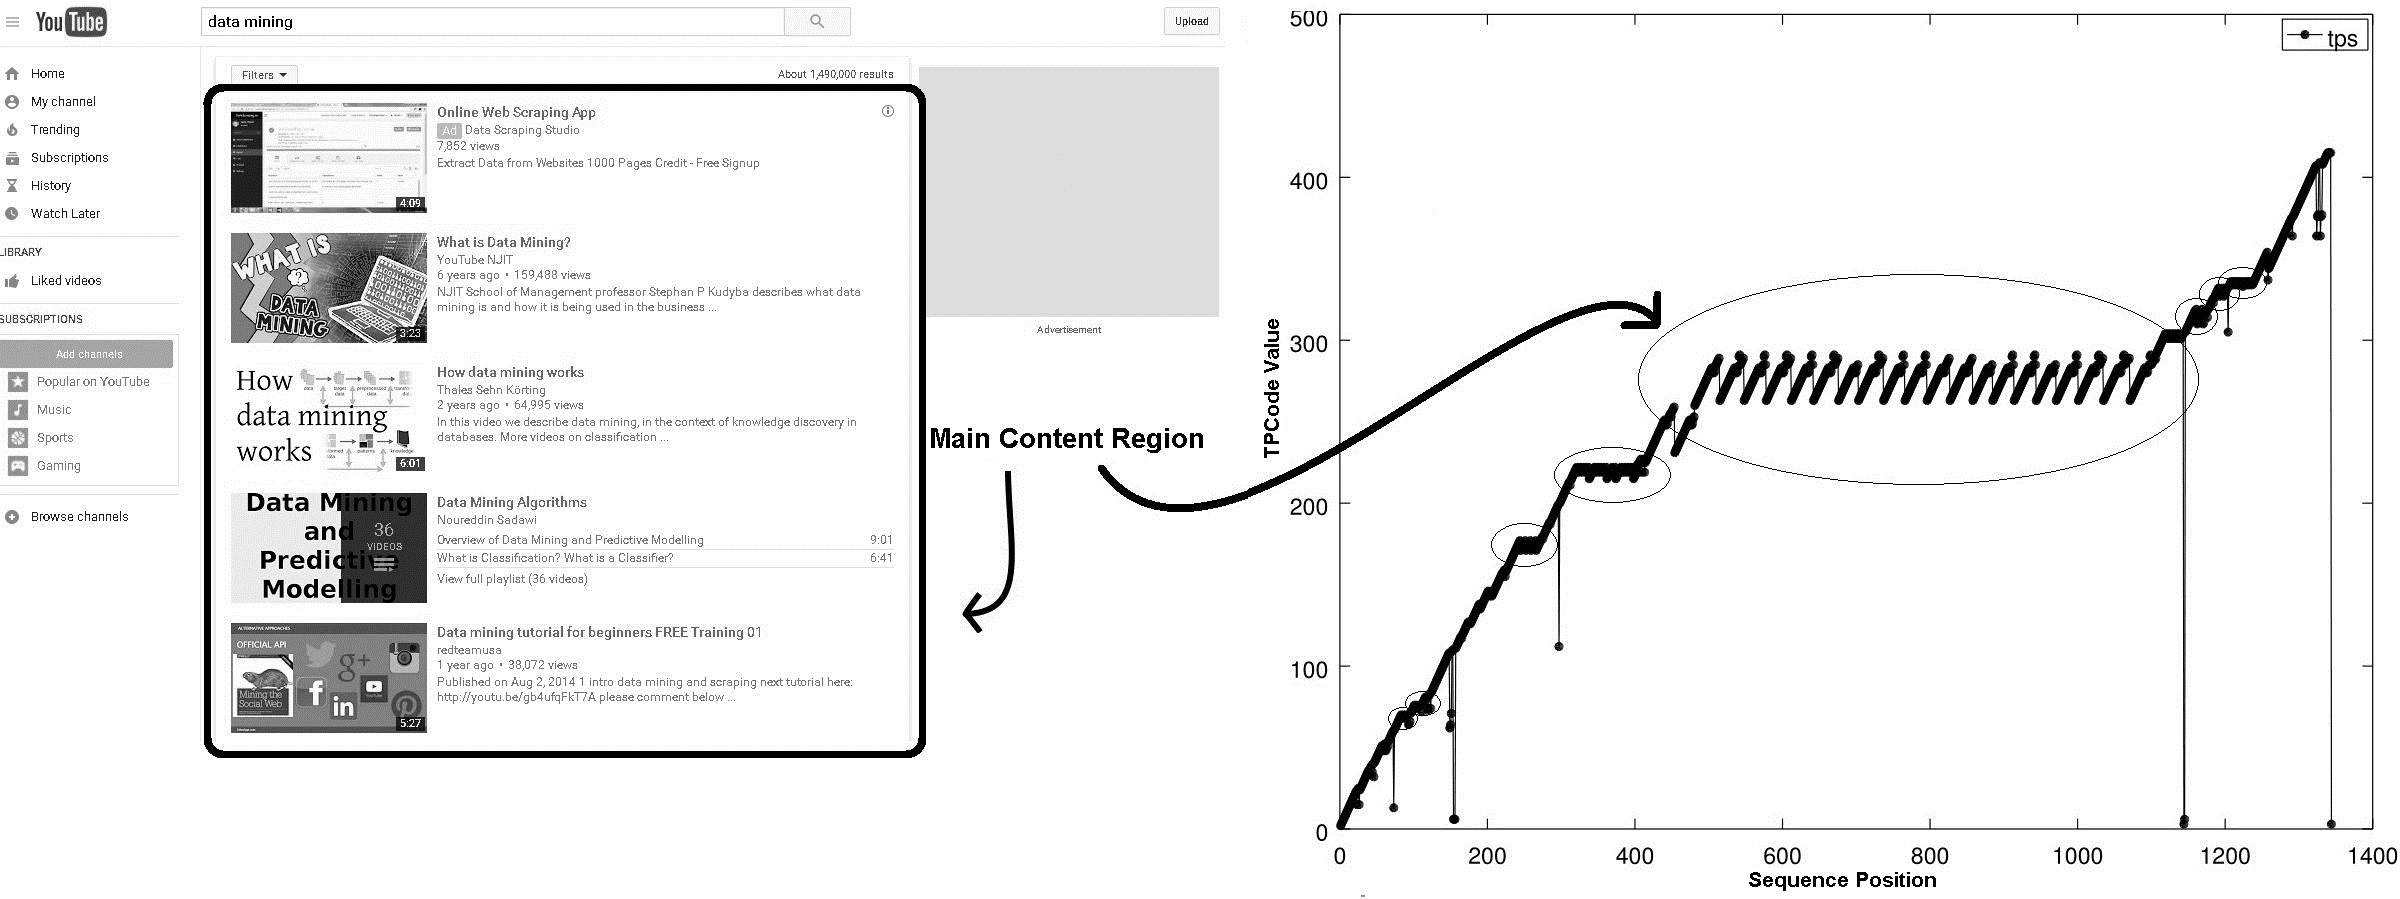
\includegraphics[width=\textwidth]{img/main-reg.jpg}}
\end{figure}
}

\frame{\frametitle{$Tag$ $paths$}
\begin{figure}[H]
  \caption{Tag Path Sequence document representation.}
  \centering
    \zoombox{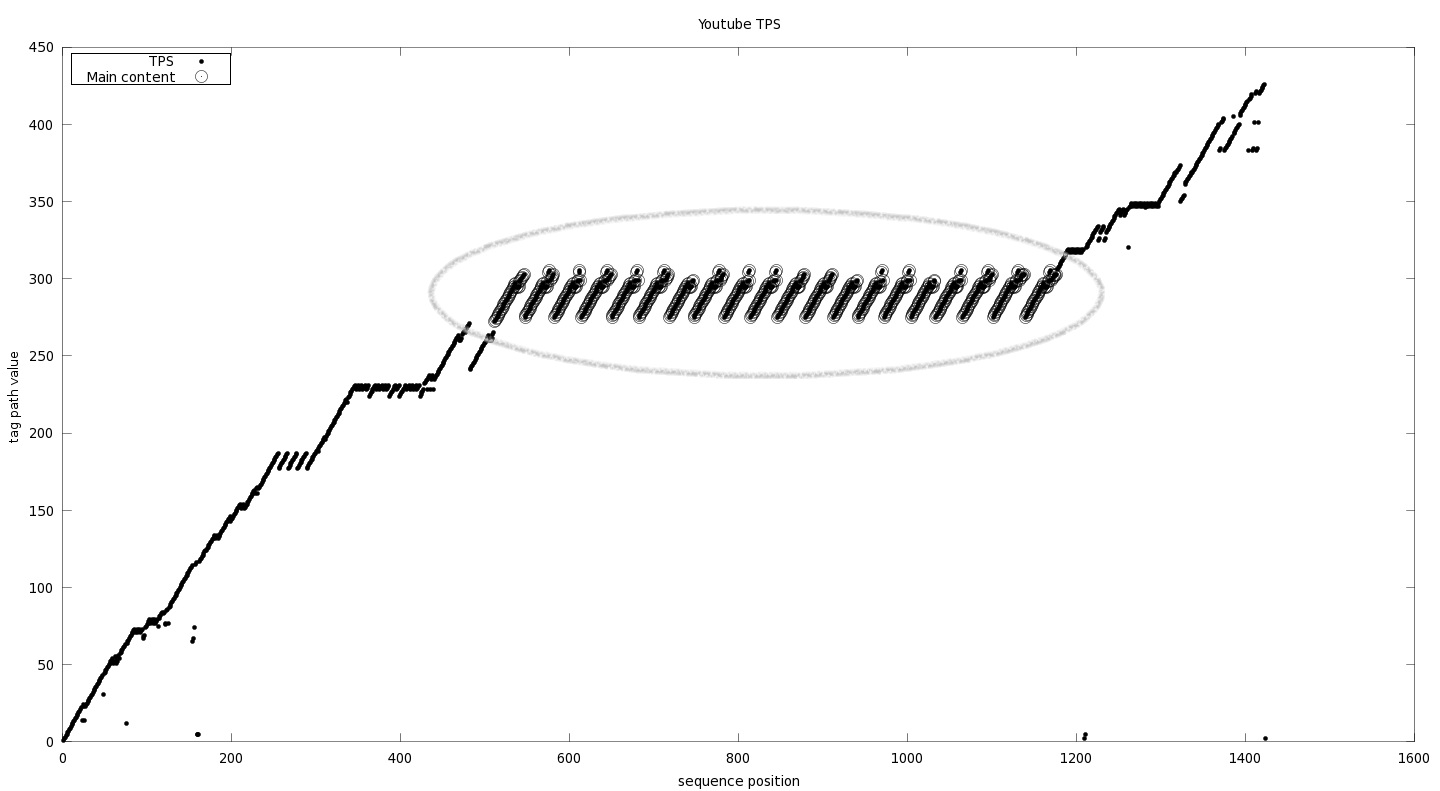
\includegraphics[width=\textwidth]{img/tps.jpg}}
\end{figure}
}

\subsection{Semi-structured Region Detection}
\frame{\frametitle{Contour}
\begin{figure}[H]
  \caption{Sequence Contour and Finite difference.}
  \centering
    \zoombox{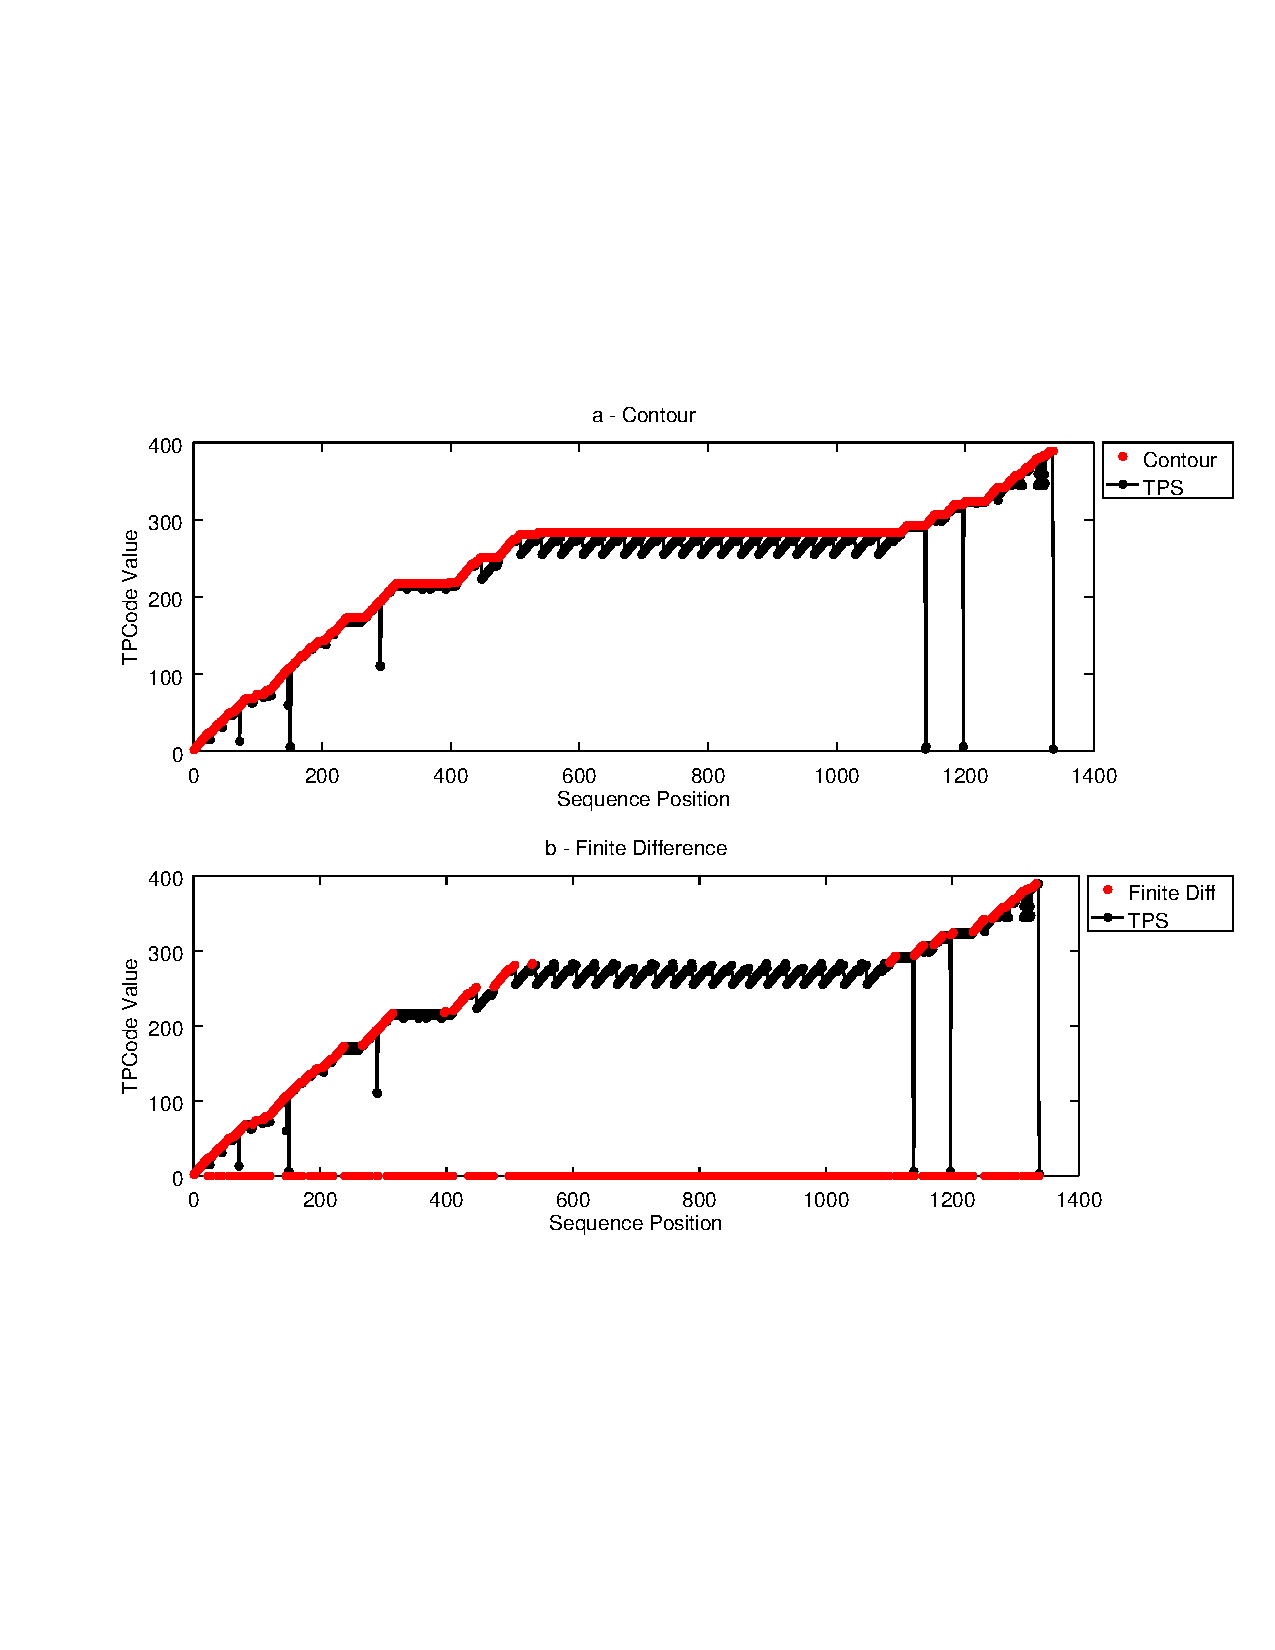
\includegraphics[trim={55 200 20
     210},clip,scale=0.45]{img/contour.pdf}}
\end{figure}
}
\subsection{Region Filtering}
\frame{\frametitle{Linear Regression}
\begin{figure}[H]
  \caption{Region's Linear Regression.}
  \centering
    \zoombox{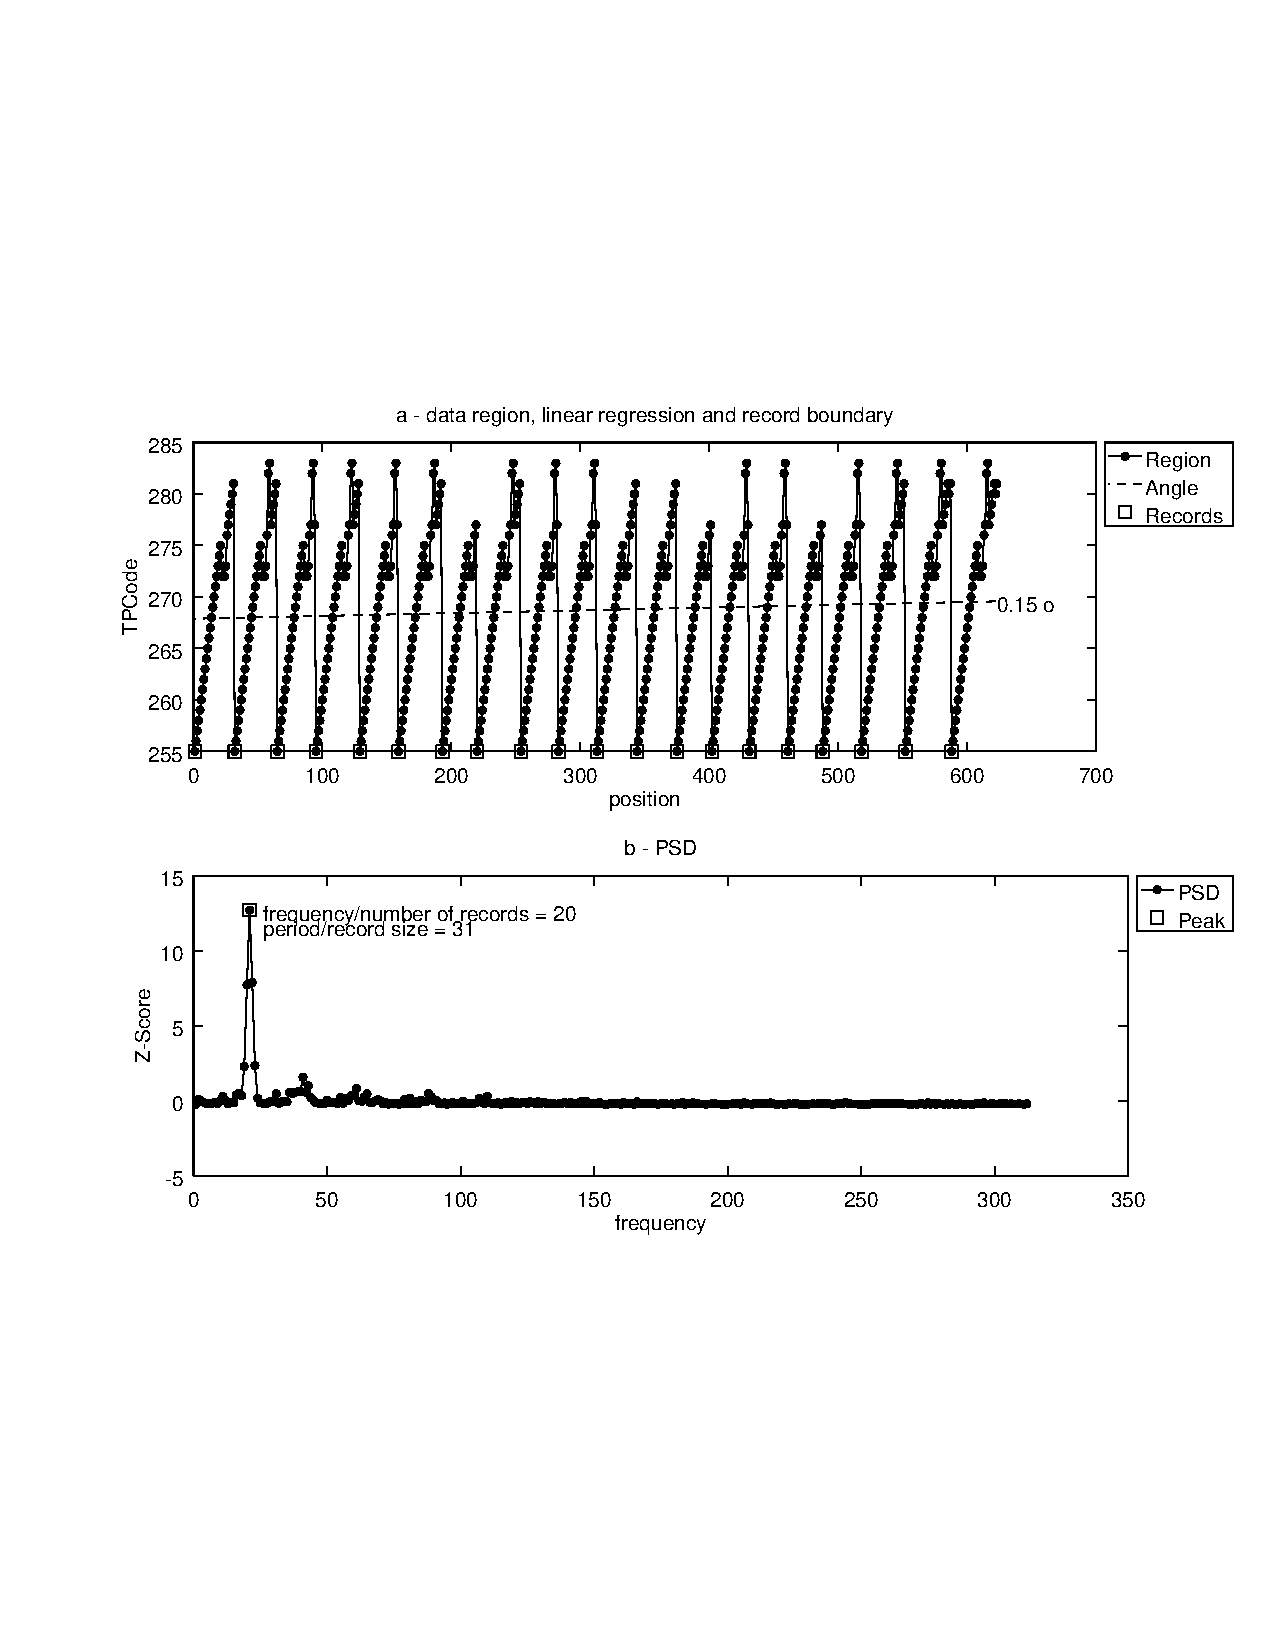
\includegraphics[trim={55 390 20
     210},clip,scale=0.45]{img/fftreg.pdf}}
\end{figure}
}

\frame{\frametitle{Clustering - Noise detection}
\begin{itemize}
\item O \textit{score} da região utilizado para clusterização é diretamente
proporcional ao tamanho da subsequência e inversamente proporcional à distância
que se encontra do centro da sequência completa;
\item É utilizado ``kmeans ótimo de uma dimensão'', forçando a criação de dois
\textit{clusters};
\item O \textit{cluster} com maior centro é considerado conteúdo e o outro
\textit{cluster} (com menor centro) é descartado.
\end{itemize}
}

\subsection{Record Identification}
\frame{\frametitle{Record count and size detection} \begin{figure}[H]
  \caption{a) TPS \& linear regression; b) PSD.}
  \centering
    \zoombox{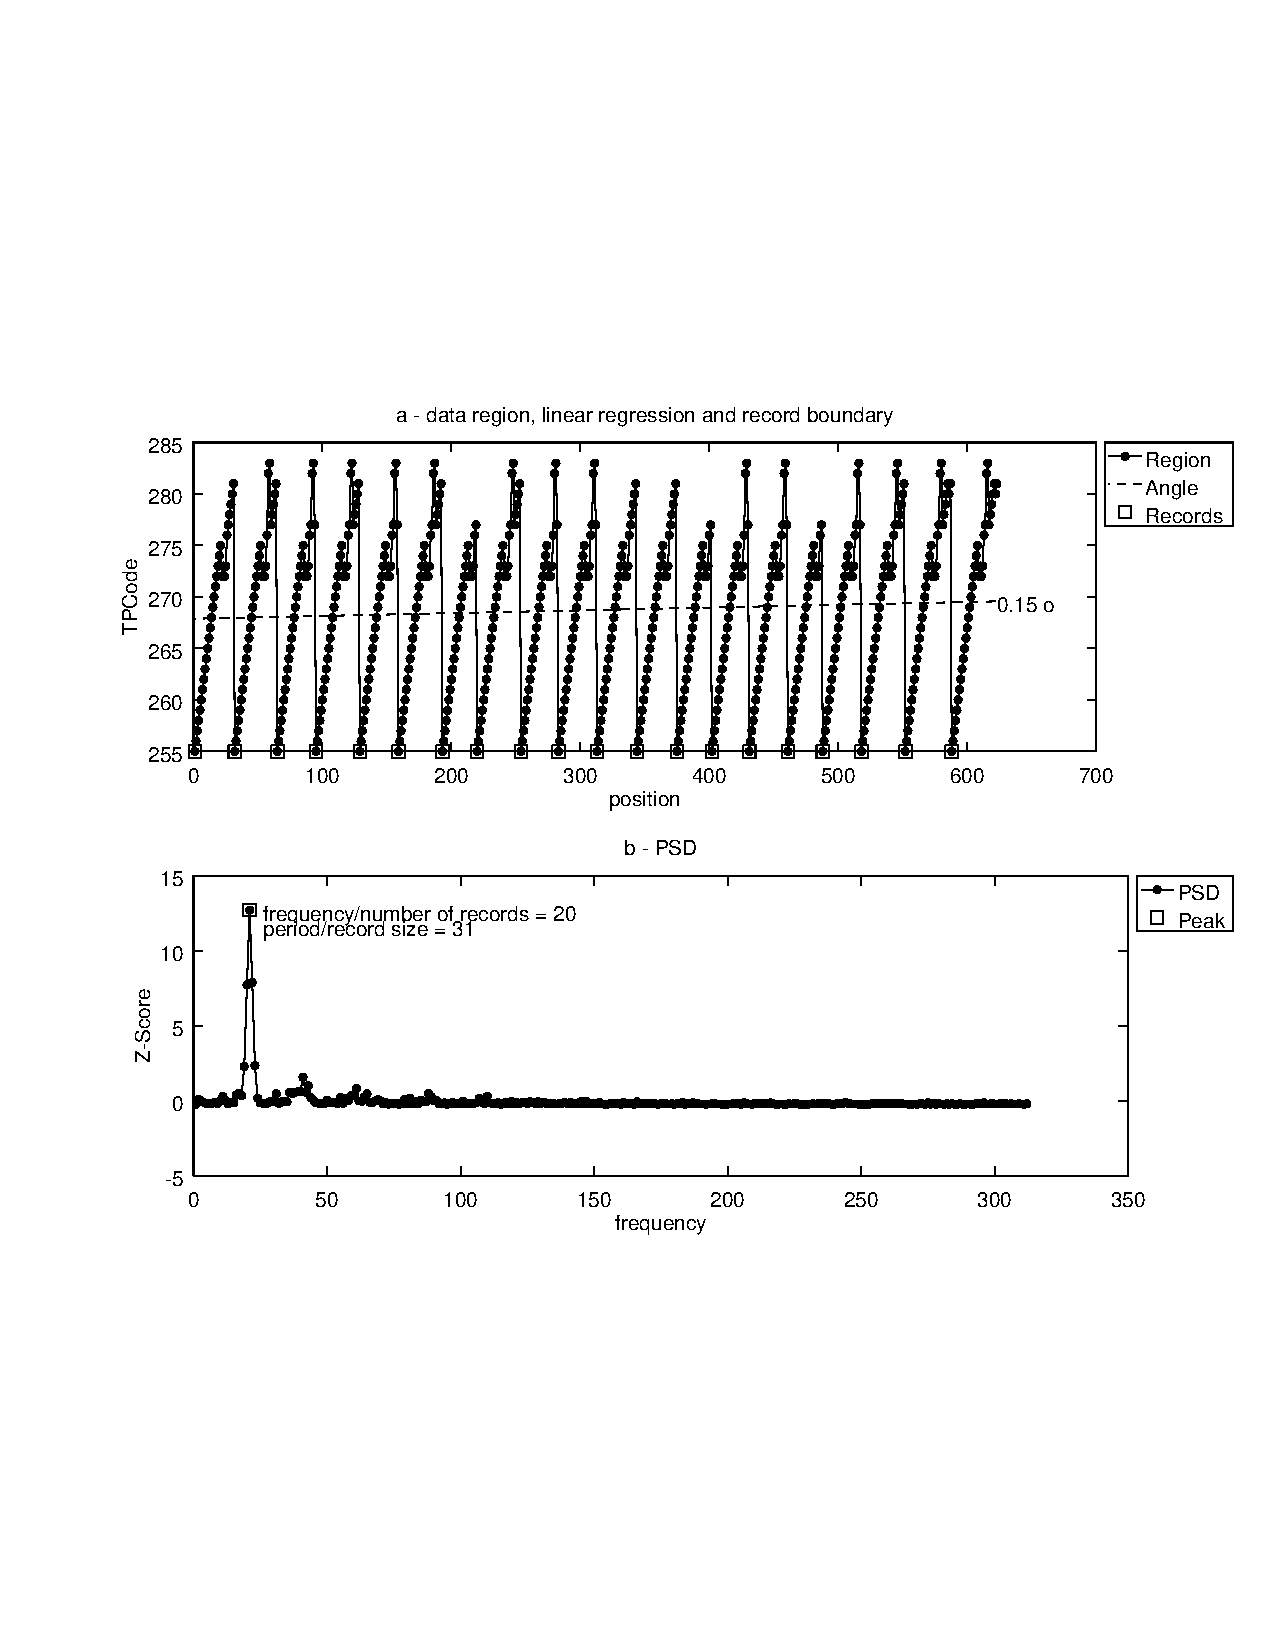
\includegraphics[clip, trim={2cm 6cm 0.5cm 6.8cm},
    width=0.8\textwidth]{img/fftreg.pdf}}
\end{figure}

} \frame{\frametitle{Detecção do tamanho e quantidade de registros - reduzindo a
complexidade computacional} Transformada de Fourier possui complexidade
$O(nlogn)$ e calcula todo o espectro do sinal. Nesta aplicação, especificamente,
apenas uma faixa do espectro é necessária. Uma alternativa, para reduzir a
complexidade, é o algoritmo de Goertzel que calcula apenas um coeficiente em
tempo linear. Outra medida (alternativa ao Z-Score) deve ser encontrada para
avaliar se um coeficiente é significativo ou não (relação de Parseval). }

\subsection{Record Alignment}
\frame{\frametitle{Center Star}
Como o alinhamento ótimo de múltiplas sequências é \textit{NP-Hard},
alternativas aproximadas, com complexidade polinomial, devem ser empregadas.

\begin{itemize}
\item Características do algoritmo \textit{Center Star}:
\begin{itemize}
  \item Não encontra necessariamente a solução ótima;
  \item Tem complexidade computacional polinomial $O(k^2\cdot n^2)$ (porém
  elevada);
  \item Garante um erro máximo com relação à solução ótima.
\end{itemize}
\end{itemize}
}

\frame{\frametitle{Solução de alinhamento específica para o problema}
As restrições do problema geral de alinhamento de múltiplas sequências não
precisam ser aplicadas, obrigatoriamente, ao problema específico de alinhamento
de múltiplos registros. Por exemplo, a ordem dos campos pode ser flexibilizada.
Soluções mais eficientes podem ser elaboradas relaxando o problema.
}

\section{Results}
\subsection{Precision, Recall \& F-Score}

\frame{\frametitle{Precision, Recall \& F-Score}
Resultados obtidos com dataset próprio contendo $1466$ registros de $46$
websites, de diversos domínios, das maiores empresas da internet:
\url{https://en.wikipedia.org/wiki/List_of_largest_Internet_companies}.

\begin{table}[h]
\centering
\begin{tabular}
{| c| c| c|}\hline
	Precision	& Recall	& F-Score\\ \hline
	98.95\% & 89.77\% & 94.13\% \\ \hline
\end{tabular}
\end{table}

Comparativo com outras técnicas estado da arte.
\begin{table}[h]
%\begin{small}
\begin{tabular}
{|c| c| c| c|}\hline
	& Precision	& Recall	& F-Score\\ \hline
MDR &	59,80\%	& 61,80\%	& 60,78\%\\ \hline
TPC	& 90,40\%	& 93,10\%	& 91,73\%\\ \hline
ClustVX &	99.81\% & 99.52\% & 99.66\%\\ \hline
Ours &	92,02\%	& 94,11\%	& 93,05\% \\ \hline
\end{tabular}
%\end{small}
%}
\end{table}


}

\subsection{Runtime analysis}
\frame{\frametitle{Tempo de execução}
\begin{figure}[h]
  \centering
     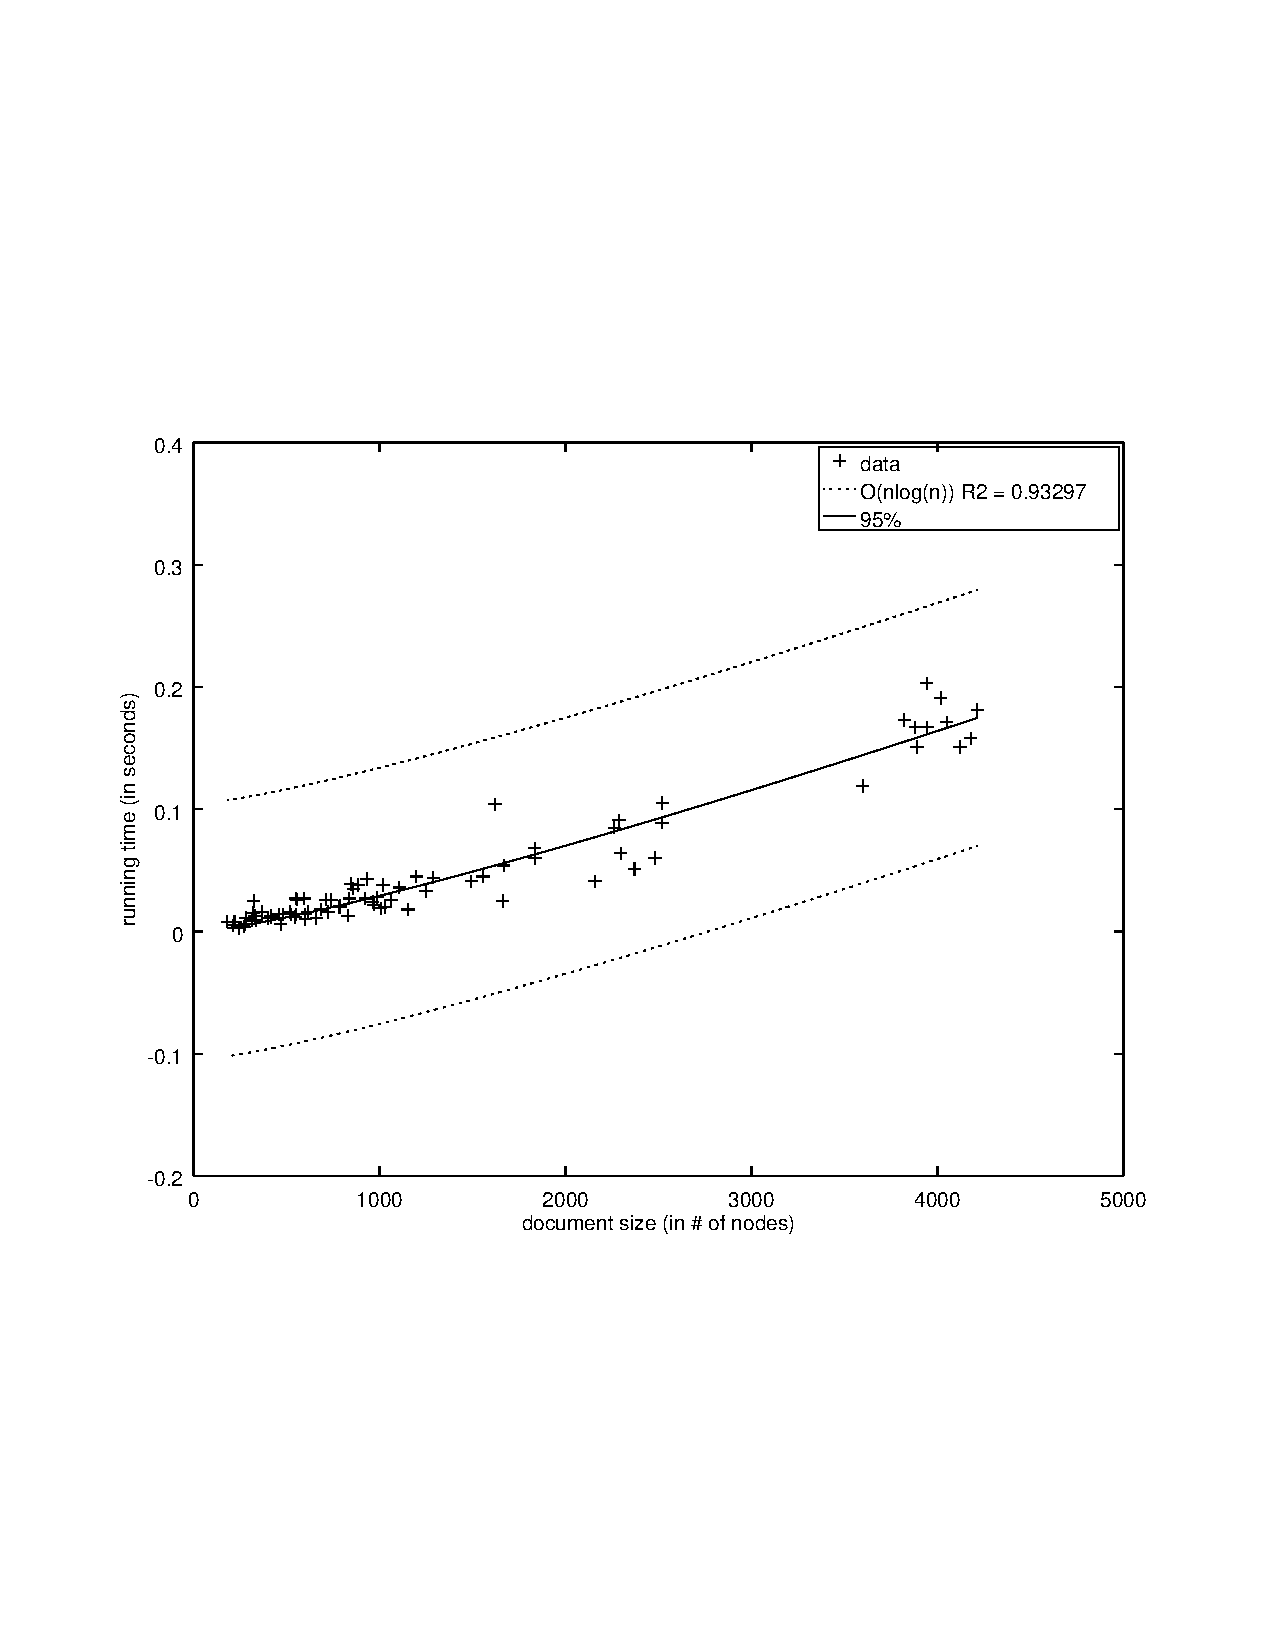
\includegraphics[clip, trim={2.0cm 7.0cm 2.0cm 7.3cm}, width=1.0\textwidth
     ]{img/runtime.pdf}
  \label{fig:runtime}
\end{figure}

}
%\frame{\frametitle{Tempo de execução}
%\begin{figure}[h]
%  \centering
%     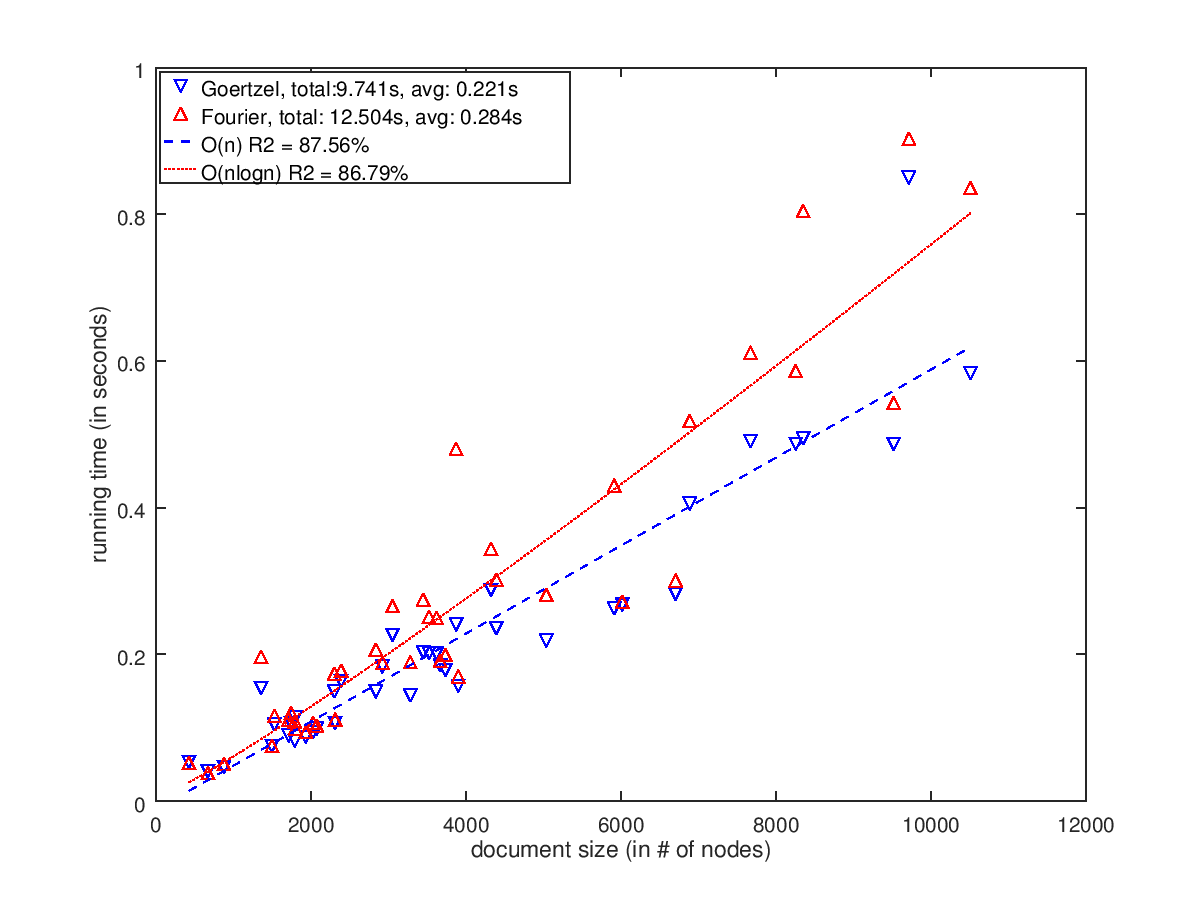
\includegraphics[width=1.0\textwidth]{img/goertzel.png}
%  \label{fig:runtime}
%\end{figure}

%}
\end{document}
